\documentclass[a4paper,12pt]{article}
\usepackage[utf8]{inputenc}

%  Русский язык
\usepackage{multirow}
\usepackage{wrapfig}
\usepackage[T2A]{fontenc}			% кодировка
\usepackage[utf8]{inputenc}			% кодировка исходного текста
\usepackage[english,russian]{babel}	% локализация и переносы

\usepackage{indentfirst} %Красная строка
\usepackage[a4paper,top=1.3cm,bottom=2cm,left=1.5cm,right=1.5cm,marginparwidth=0.5cm]{geometry}
\usepackage[usenames]{color}
\usepackage{colortbl}
\usepackage{csvsimple}
\usepackage{siunitx}

\addto\captionsrussian{\def\refname{5   Список используемой литературы}}

% Заметки
\usepackage{todonotes}

% Математика
\usepackage{amsmath,amsfonts,amssymb,amsthm,mathtools} 
\usepackage{hyperref}


\usepackage{euscript}	 % Шрифт Евклид
\usepackage{mathrsfs} % Красивый матшрифт


\renewcommand{\AA}{\ensuremath{\mathring{A}}}

\begin{document}
\def\figurename{Рисунок}
\begin{titlepage}
\begin{center}
    {\large МОСКОВСКИЙ ФИЗИКО-ТЕХНИЧЕСКИЙ ИНСТИТУТ (НАЦИОНАЛЬНЫЙ ИССЛЕДОВАТЕЛЬСКИЙ УНИВЕРСИТЕТ)}
\end{center}
\begin{center}
    {\largeФизтех-школа биологической и медицинской физики}
\end{center}

\vspace{1cm}
{\huge
\begin{center}
    {\bf Лабораторная работа по физической химии}\\
    \vspace{0.5cm}
    Адсорбция и мицеллообразование в растворах ПАВ: определение ККМ по измерению электропроводности и поверхностного натяжения
\end{center}
}

\vspace{4cm}
\begin{flushright}
{\LARGE Выполнила студентка группы Б06-103:\\ Фитэль Алена \\}

\end{flushright}
\vspace{9cm}
\begin{center}
    Долгопрудный, 2023 г.
\end{center}
\end{titlepage}
\newpage
\newpage
\section{Введение}
\setcounter{page}{2}
\textbf{Цели работы}: 
\begin{itemize}
    \item Освоение методик определения критической концентрации мицеллообразования
ионогенных и неионогенных ПАВ по измерениям электропроводности и
поверхностного натяжения растворов.
    \item Оценка степени ионизации мицелл ионогенных ПАВ по результатам
кондуктометрических измерений.
    \item Построение изотермы поверхностного натяжения и адсорбции ПАВ на поверхности
раствор/воздух. Определение площади, занимаемой молекулой ПАВ в насыщенном
адсорбционном слое.
    \item Исследование влияния температуры и электролитов на мицеллообразование в
растворах ПАВ.
\end{itemize}
\section{Теоретические сведения}
\subsection{Кондуктометрический метод}
Рассмотрим зависимость удельной электропроводности $\varkappa$ от концентрации ионогенного ПАВ на примере SDS (анионный ПАВ):

\begin{itemize}

\item При С<ККМ мицеллы не образуются:

\begin{equation}\label{c<ккм}
        \varkappa = \lambda_{Na}  [Na^{+}] + \lambda_{DS}  [DS^{-}] = (\lambda_{Na} + \lambda_{DS}) [SDS]
\end{equation}

где $\lambda_{Na},\lambda_{DS}$ - соответствующие эквивалентные электропроводности.

\item При C > ККМ начинают образовываться мицеллы.

\begin{equation}\label{eq1}
    \varkappa = \lambda_{Na}  [Na^{+}] + \lambda_{DS}  [DS^{-}] + \lambda_{mic} [mic^{-}]
\end{equation}

где: $[Na^{+}]$, $[DS^{-}]$ - концентрации свободных ионов (не в мицелле), $[mic^{-}]$ - концентрация мицелл. 
Пусть:
\begin{itemize}
    \item N - число агреаций (количество молекул, из которых образуется 1 мицелла ПАВ)\
    \item  M - число $Na^{{+}}$, связанных с мицеллой. Тогда заряд мицеллы $-(N - M)$\
    \item  $\alpha = \frac{N - M}{N}$ - cтепень ионизации мицеллы
\end{itemize}
Тогда: \begin{itemize}
    \item $[DS^{-}] = \text{ККМ}$
    \item $[Na^{+}] = \text{ККМ} + \alpha N [mic^{-}]$, где $\alpha N [mic^{-}]$ - число $[Na^{+}]$, не связанных с мицеллами
    \item $\lambda_{mic} = \alpha N \lambda_{DS}$, так как $\alpha N$ - число $DS^{-}$ в мицелле, не связанных с $Na^{+}$
    \item $[mic^{-}] = \frac{[SDS] - \text{ККМ}}{N}$, так как $[SDS]$ - полная концентрация молекул ПАВ, $\text{ККМ}$ - концентрация сводобных молекул ПАВ. На $N$ делим потому, что в 1 мицелле N молекул ПАВ
\end{itemize}


Подставляя полученные выражения в (\ref{eq1}) получаем:
 \begin{equation*}
    \varkappa = \lambda_{Na} (\text{ККМ} + \alpha N \frac{[SDS] - \text{ККМ}}{N}) +  \lambda_{DS} \text{ККМ} + \alpha N \lambda_{DS} \frac{[SDS] - \text{ККМ}}{N} =
\end{equation*}
\begin{equation*}
    = [SDS]\alpha(\lambda_{Na} + \lambda_{DS}) + \text{ККМ} (\lambda_{Na} - \alpha \lambda_{Na} + \lambda_{DS} - \alpha \lambda_{DS}) = 
\end{equation*}
\begin{equation*}
    = [SDS]\alpha(\lambda_{Na} + \lambda_{DS}) + (1 - \alpha)\text{ККМ}(\lambda_{Na} + \lambda_{DS})
\end{equation*}
В итоге при С > ККМ
\begin{equation}\label{c>ккм}
    \varkappa = [SDS]\alpha(\lambda_{Na} + \lambda_{DS}) + (1 - \alpha)\text{ККМ}(\lambda_{Na} + \lambda_{DS})
\end{equation}
\end{itemize}
Значит, график зависимости $\varkappa(C)$ выглядит следующим образом (уравнение (\ref{c<ккм}) при C<ККМ и  (\ref{c>ккм}) при С>ККМ)\\
\begin{figure}[h!]
    \centering
    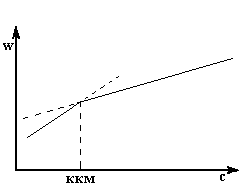
\includegraphics[width = 0.3\textwidth]{cele.png}
    \caption{График зависимости удельной электропроводности W от концентрации ПАВ (уравнение (\ref{c<ккм}) при C<ККМ и уравнение (\ref{c>ккм}) при С>ККМ)}
    \label{fig:no_int}
\end{figure}\\
Таким образом, измерив удельную электропроводность ПАВ от концентрации, мы сможем найти ККМ по излому получившегося графика

\subsection{Метод измерения поверхностного натяжения раствора ПАВ}
Рассмотрим зависимость поверхностного натяжения ПАВ (ионогенного или неионогенного) от концентрации.\ 
Вспомогательные сведения:
\begin{itemize}
    \item Адсорбция - это изменение концентрации вещества в растворе вблизи поверхности 
    \item Поверхностный избыток $\text{Г} = \frac{N_{d} - N}{S}$, где $N_{d}$ - число молекул вещества вблизи поверхности раздела фаз, $N$ - число молекул вещества в глубине раствора, $S$ - площадь поверхности раздела фаз
    \item Изотерма адсорбции Ленгмюра. В данной теории используются следующие приближения:
    \begin{itemize}
        \item молекулы растворенного вещества взаимодействуют с активными центрами на поверхности раздела фаз
        \item адсорбированные молекулы образуют монослой на поверхности раздела фаз
        \item нет взаимодействия между соседями в монослое
    \end{itemize}
    Уравнение адсорбции Ленгмюра
    \begin{equation} \label{ленгмюр}
        \text{Г} = \text{Г}_{\infty}\frac{KC}{KC + 1}
    \end{equation}
    где $\text{Г}_{\infty}$ - предельное значение адсорбции (когда все активные центры заняты), С - концентрация адсорбирующегося вещества в глубине раствора, К - константа 
    \item Поверхностное натяжение - это работа образования единицы площади поверхности (границы раздела фаз)
    \item Коэффициент поверхностного натяжения - сила, действующая на единицу длины линии, ограничивающей поверхность жидкости
    \begin{equation} \label{sigma}
        \sigma = \frac{F_{\text{пов}}}{l}
    \end{equation} 
    \item Уравнение Гиббса:
    \begin{equation}\label{гиббс}
        \text{Г} = -\frac{C}{RT} \frac{d\sigma}{dC} = - \frac{1}{RT} \frac{d\sigma}{dlnC}
    \end{equation}\label{g}
    \item Поверхностная активность (при $C \rightarrow 0$)
    \begin{equation}
        g = -\frac{d\sigma}{dC}
    \end{equation}
    У ПАВ $g > 0$.
\end{itemize}
Подставим в (\ref{гиббс}) уравнение (\ref{ленгмюр}):
\begin{equation*}
    d\sigma = -\text{Г} R T dC = -\frac{KC}{KC + 1} \text{Г}_{\infty} R T dlnC = -\text{Г}_{\infty}RT\frac{d(1 + KC)}{(1 + KC)}
\end{equation*}
Получим уравнение Шишковского:
\begin{equation}
    \sigma = \sigma_{0} - \text{Г}_{\infty}RTln(KC + 1)
\end{equation}

Построим уравнение (\ref{гиббс}) в полулогарифмических координатах

\begin{figure}[h!]
    \centering
    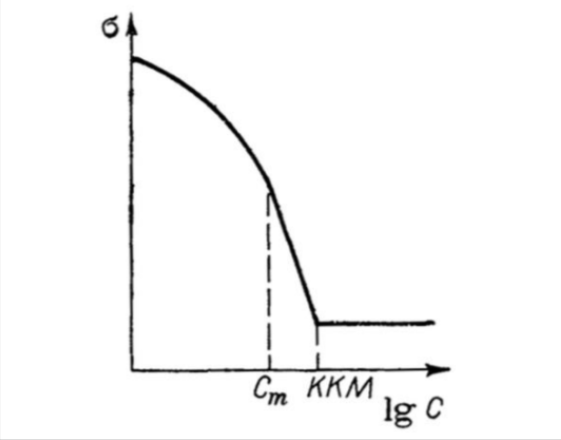
\includegraphics[width = 0.4\textwidth]{natyazh.png}
    \caption{График зависимости коэффициента поверхностного натяжения от логарифма концентрации ПАВ}
    \label{fig:теорln}
\end{figure}

$C_{m}$ - пороговая концентрация, выше которой $\text{Г} = \text{Г}_{\infty}$ (адсорбционный слой становится насыщенным)\ 
Все вышесказанное работает при концентрациях ниже ККМ, так как при С>ККМ концентрация свободных частиц в растворе перестает меняться и $\sigma = const$ \\
Таким образом, измерив поверхностное натяжение ПАВ от концентрации, мы сможем найти ККМ по излому получившегося графика.
\subsubsection{Метод пластины Вильгельма}
 Для определения коэффициента поверхностного натяжения в данной работе используется метод пластины Вильгельма. Методика эксперимента:
\begin{itemize}
    \item опускаем небольшую пластинку, подвешенную к весам, в раствор заданной концентрации
    \item измеряем $\Delta m $ пластинки в жидкости и свободно подвешенной
    \item для измерения массы пластинки в жидкости пластинка с помощью специального механизма медленно опускается к краю жидкости до касания 
\end{itemize}

\begin{figure}[h!]
    \centering
    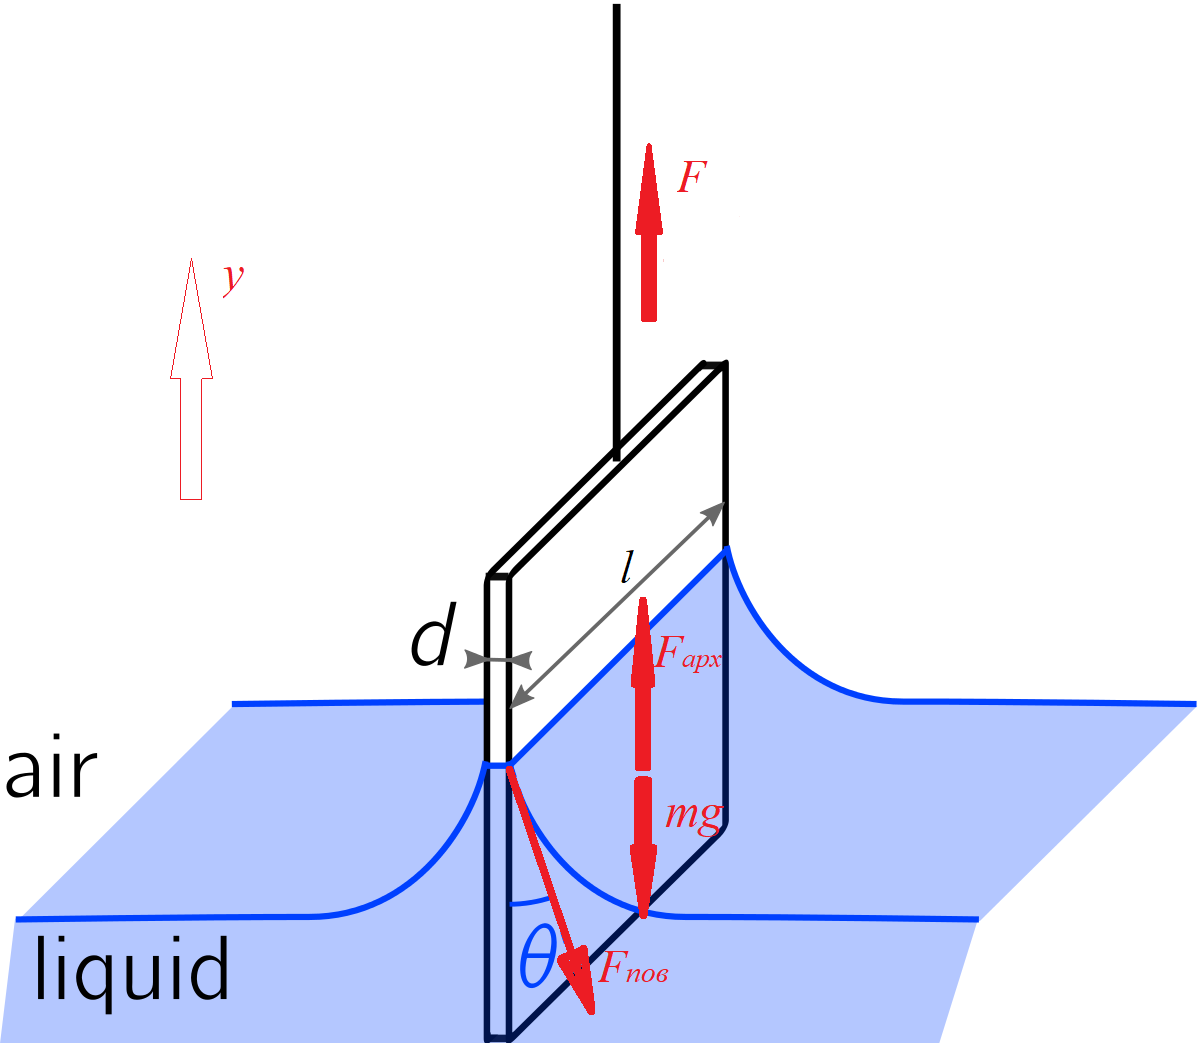
\includegraphics[width = 0.5\textwidth, height = 70mm]{Wilhelmy_plate.png}
    \caption{Схема установки по методу пластины Вильмельма}
    \label{fig:no_int}
\end{figure}
Распишем силы, действующие на пластинку вне жидкости ($F_{1}$) и в жидкости ($F_{2}$)\
\begin{equation*}
    y: F_{1} - mg = 0
\end{equation*}
\begin{equation*}
    y: F_{2} - mg + F_{\text{арх}} - F_{\text{пов y }} = 0
\end{equation*}
\begin{equation*}
    F_{2} - F_{1} = \Delta F  = F_{\text{пов y }} - F_{\text{арх}}
\end{equation*}
Сила Архимеда 
\begin{equation*}
    F_{\text{арх}} = \rho V_{\text{погр в жидк}} g = \rho x l d g
\end{equation*}
где $\rho$ - плотность жидкости.\\
Считаем, что при аккуратном проведении опыта $x \approx 0$, поэтому силой Архимеда можно пренебречь.\\
Сила поверхностного натяжения (из (\ref{sigma})) :
\begin{equation*}
    F_{\text{пов y }} = F_{\text{пов}}cos(\theta) = 2\sigma(d + l)cos(\theta)
\end{equation*}
где $\theta$ - угол смачивания\\
Для того, чтобы не рассчитывать угол смачивания, возьмем поверхность пластинки с полным смачиванием (стекло), т.е $\theta = 0, cos(\theta) = 1$\\
С учетом $d \ll l$ получим
\begin{equation*}
    F_{\text{пов y }} = 2\sigma
\end{equation*}
Тогда \begin{equation*}
    \Delta F = 2 \sigma l
\end{equation*}
\begin{equation}
    \sigma = \frac{9.8 \Delta m}{2l}, \hspace{1 cm} [\sigma] = \frac{\text{мН}}{\text{м}}, \hspace{1 cm} [\Delta m] = \text{г}, \hspace{1 cm} [l] = \text{м}.
\end{equation}
\section{Ход работы и обработка данных}
\subsection{Используемое ПАВ в работе}

В данной работе был использован катионный ПАВ TTAB(тетрадецилтриметиламмоний бромид).

\begin{figure}[h!]
    \centering
    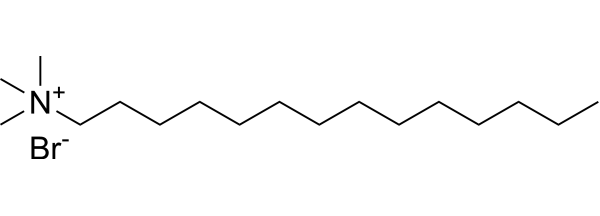
\includegraphics[width = 0.4\textwidth]{55.png}
    \caption{TTAB(тетрадецилтриметиламмоний бромид)}
    \label{fig:no_int}
\end{figure}

Ожидаемое значение ККМ TTAB \cite{1}:
\begin{equation}
    {\text{ККМ}} = 3.5 {\text{ мМ}}
\end{equation}
Ожидаемое значение числа агрегаций TTAB \cite{1}: 
\begin{equation}
    N = 75
\end{equation}

\subsection{Определение ККМ в растворе ПАВ кондуктометрическим методом}
Для выполнения работы использовались растворы
катионного ПАВ тетрадецилтриметиламмония бромида (TTAB) в различных концентрациях. После измерения удельной электропроводности чистой воды и всех приготовленных растворов были получены данные, которые представлены в  Таблице 1 (погрешности ).   По полученным данным был построен график зависимости удельной электропроводности от концентрации раствора (Рисунок 5).

\begin{table}[h!]
\centering
\begin{tabular}{|r|r|r|r|r|}
\hline
\multicolumn{1}{|l|}{№} & \multicolumn{1}{l|}{C, мМ} & \multicolumn{1}{l|}{$\varkappa_{down}$, мкСм/см} & \multicolumn{1}{l|}{C, мМ} & \multicolumn{1}{l|}{$\varkappa_{up}$, мкСм/см} \\ \hline
1                       & 10.5                       & 517                                              & 0.35                       & 42.8                                           \\ \hline
2                       & 9.275                      & 489                                              & 0.98                       & 112                                            \\ \hline
3                       & 8.05                       & 461                                              & 1.61                       & 183                                            \\ \hline
4                       & 6.825                      & 433                                              & 2.24                       & 252                                            \\ \hline
5                       & 5.6                        & 403                                              & 2.87                       & 323                                            \\ \hline
6                       & 4.375                      & 371                                              & 3.5                        & 378                                            \\ \hline
7                       & 3.5                        & 333                                              & 4.375                      & 419                                            \\ \hline
8                       & 2.87                       & 286                                              & 5.6                        & 458                                            \\ \hline
9                       & 2.24                       & 227                                              & 6.825                      & 492                                            \\ \hline
10                      & 1.61                       & 165.1                                            & 8.05                       & 524                                            \\ \hline
11                      & 0.98                       & 103.7                                            & 9.275                      & 555                                            \\ \hline
12                      & 0.35                       & 38                                               & 10.5                       & 588                                            \\ \hline
\end{tabular}
\caption{Результаты измерения удельной электропроводности кондуктометрическим методом.}
\label{tab:my-table}
\end{table}

\begin{figure}[h!]
    \centering
    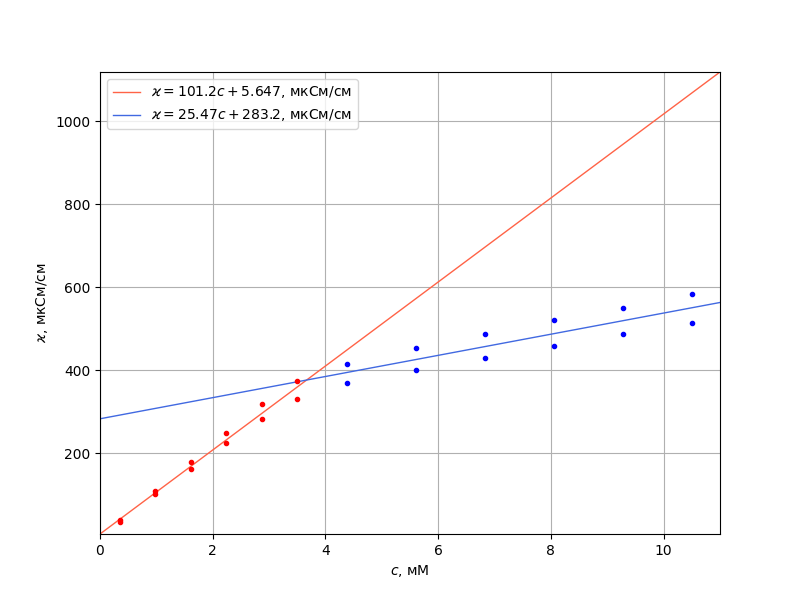
\includegraphics[width = 0.65\textwidth]{data 1.png}
    \caption{График зависимости удельной электропроводности от концентрации ПАВ. }
    \label{fig:no_int}
\end{figure}

        
 Излом графика соответствует критической концентрации мицелообразования - 3.67 мМ. Степень ионизации мицелл определяется отношением наклонов
зависимостей $\kappa$ от полной концентрации $TTAB$ и численно равна:
$\alpha = \frac{k_2}{k_1} = \frac{25.47}{101.2} = 0.090$.

\subsection{Определение ККМ методом измерения поверхностного натяжения}
В данной части работы измерено поверхностное натяжение 12 растворов, используя метод пластины Вильгельми с помощью весов.
\begin{enumerate}
    \item Снимем показания весов при различный концентрациях раствора TТАВ, а затем рассчитаем поверхностное натяжение, занесем результаты в Таблицу 2. Построим график зависимости поверхностного натяжения от концентрации раствора (Рисунок 6, Рисунок 7).

\begin{table}[h!]
\centering
\begin{tabular}{|c|r|r|r|}
\hline
№  & \multicolumn{1}{l|}{$c$, мМ} & \multicolumn{1}{l|}{$\ln{c}$} & \multicolumn{1}{l|}{$\sigma$, мН/м} \\ \hline
1  & 8.751                        & 2.16916798                    & 36.09618815                         \\ \hline
2  & 6.563                        & 1.881447815                   & 35.56208919                         \\ \hline
3  & 4.375                        & 1.47590652                    & 33.38118509                         \\ \hline
4  & 3.508                        & 1.255046075                   & 31.91241295                         \\ \hline
5  & 3.126                        & 1.139754232                   & 31.02224801                         \\ \hline
6  & 2.744                        & 1.00941671                    & 30.44364081                         \\ \hline
7  & 2.362                        & 0.8595087178                  & 30.88872327                         \\ \hline
8  & 1.98                         & 0.6830968447                  & 34.84995724                         \\ \hline
9  & 1.216                        & 0.1955667835                  & 41.659719                           \\ \hline
10 & 0.834                        & -0.1815218766                 & 46.37759316                         \\ \hline
11 & 0.452                        & -0.7940730991                 & 55.19022602                         \\ \hline
12 & 0.07                         & -2.659260037                  & 65.69417227                         \\ \hline
\end{tabular}
\caption{Поверхностное натяжение в зависимости от концентрации ПАВ}
\label{tab:my-table}
\end{table}

\begin{figure}[h!]
    \centering
    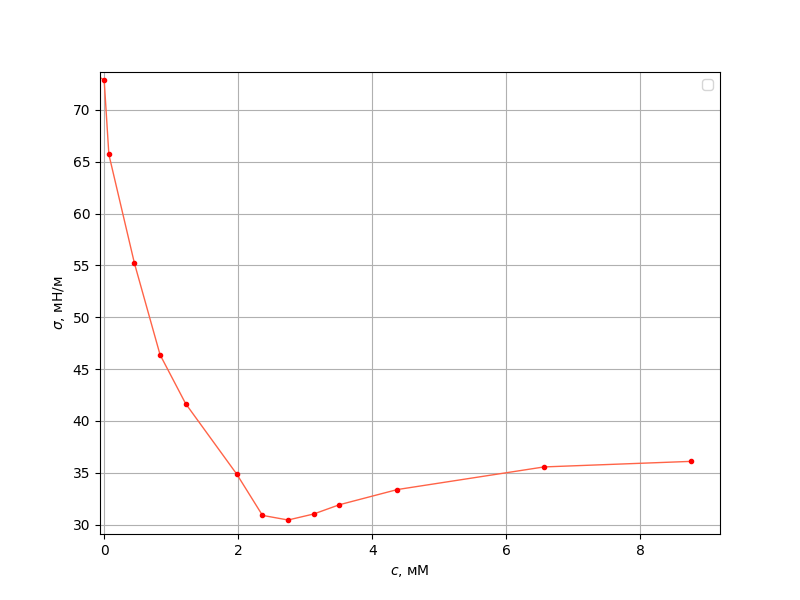
\includegraphics[width = 0.7\textwidth]{Figure_1.png}
    \caption{Зависимость поверхностного натяжения от концентрации ПАВ.}
\end{figure}

\begin{figure}[h!]
    \centering
    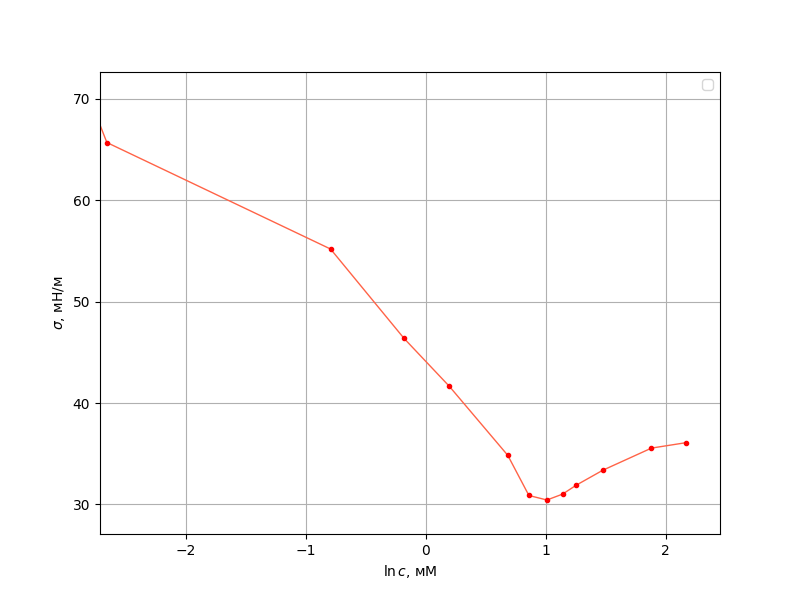
\includegraphics[width = 0.7\textwidth]{sigma_ln(c).png}
    \caption{Зависимость поверхностного натяжения от концентрации ПАВ в полулогарифмических координатах.}
\end{figure}\\


\item
В отличие от теоретического графика(Рисунок 2) на полученной зависимости (Рисунок 7) есть минимум. Его появление можно объяснить тем, что в растворе были примеси, обладающие большей поверхностной активностью, чем TTAB. Так как примеси более поверхностно активны, то они лучше адсорбируются  на поверхности, и, следовательно, поверхностное натяжение уменьшается.
\item
Для приблизительной оценки значения ККМ  проведем 2 прямые, на пересечении которых должна получиться ККМ (согласно теории)(Рисунок 8)\\

\begin{figure}[h!]
    \centering
    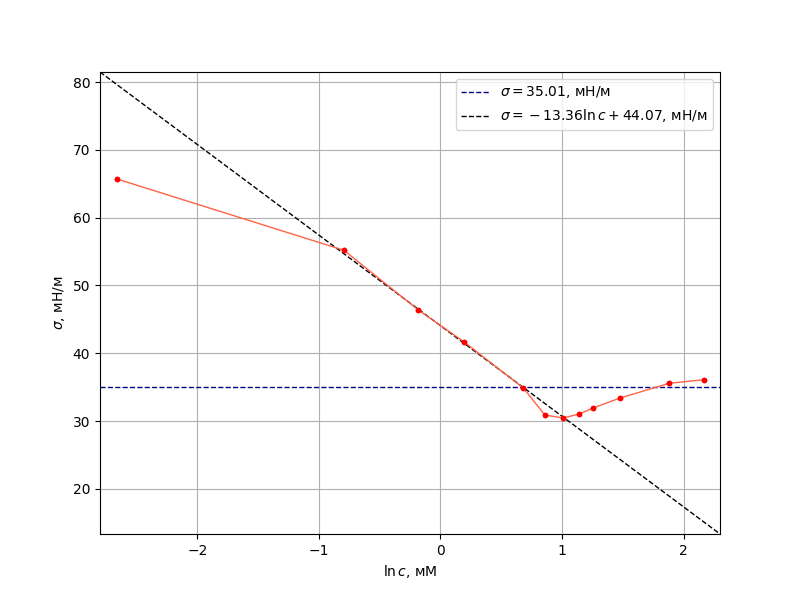
\includegraphics[width = 0.7\textwidth]{sigma_approx.png}
    \caption{Зависимость поверхностного натяжения от концентрации ПАВ в полулогарифмических координатах, аппроксимация предельных точек прямыми.}
\end{figure}\\

Прямые пересекаются при:
\begin{equation*}
    ln(\text{ККМ}) = 0.678 \Rightarrow \text{ККМ} = 1.97 \text{мМ}
\end{equation*}

Полученное значение ККМ слабо согласуется с теоретическим.
\item
Определим предельное значение адсорбции $\text{Г}_{\infty}$ по наклону прямолинейного участка графика перед предельным участком. Из уравнения Гиббса (\ref{гиббс}):
\begin{equation*}
    \text{Г}_{\infty} = - \frac{1}{RT} \frac{d\sigma}{dlnC}
\end{equation*}
Из полученного графика в полулогарифмических координатах():  \\
\begin{equation*}
    \frac{d\sigma}{dlnC} = - 13.36 \cdot 10^{-3} \frac{H}{\text{м}}
\end{equation*}\\
Температура в лаборатории: $T = 298 K$, тогда:
\begin{equation*}
    \text{Г}_{\infty} = - \frac{1}{8.31 \cdot 298} \cdot (- 13.36 \cdot 10^{-3}) \frac{\text{моль}}{\text{м}^{2}} = 5.39 \cdot 10^{-6} \frac{\text{моль}}{\text{м}^{2}}
\end{equation*}

\item Определим площадь, приходящуюся на одну молекулу в монослое ($N_{a} = 6.02 \cdot 10^{23} \text{моль}^{-1}$)
\begin{equation*}
    S_{0} = \frac{1}{N_{a} \text{Г}_{\infty}} = \frac{1}{6.02\cdot10^{23}\cdot 5.39\cdot10^{-6}} \text{м}^{2} = 3.08\cdot10^{-19}\text{м}^{2}
\end{equation*}

\item Оценим длину молекулы в монослое $l$. Рассмотрим объем $\nu$ молей монослоя
\begin{equation*}
    V = N S_{0} l 
\end{equation*}

С другой стороны, если d - плотность монослоя ($d = 1 \frac{\text{г}}{\text{см}^{3}}$, M - молярная масса TTAB ($M = 256.5 \frac{\text{г}}{\text{моль}}$)
\begin{equation*}
    V = \frac{m}{d} = \frac{\nu M}{d} = \frac{NM}{N_{a}d}
\end{equation*}
Тогда: 
\begin{equation*}
    S_{0}l = \frac{M}{N_{a}d} \Rightarrow l = \frac{M}{N_{a}S_{0}d} = \frac{M\text{Г}_{\infty}}{d}
\end{equation*}

\begin{equation*}
    l = \frac{256.5 \frac{\text{г}}{\text{моль}} \cdot 5.39\cdot10^{-6} \frac{\text{моль}}{\text{м}^{2}}}{ \frac{1\text{г}}{10^{-6}\text{м}^{3} }}} = 1.38 \cdot 10^{-9} \text{м}
\end{equation*}

Сравним полученное значение $l$ с геометрической оценкой \cite{2}:
\begin{figure}[h!]
    \centering
    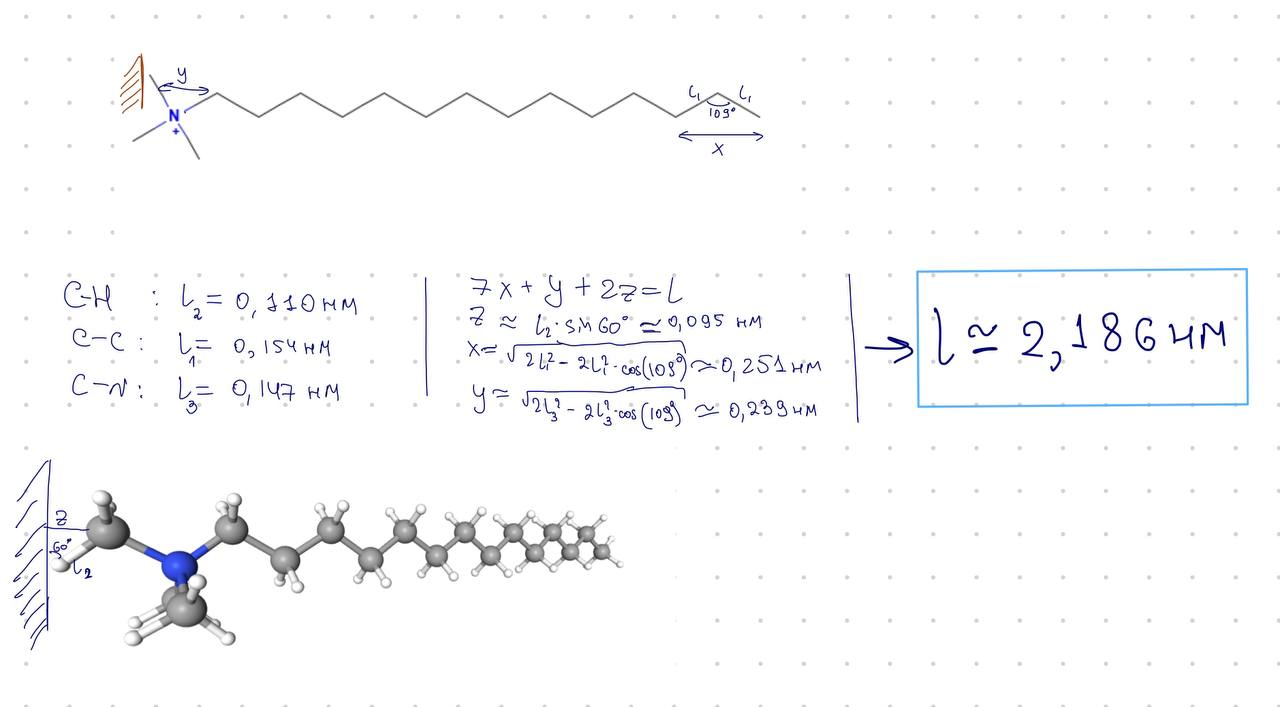
\includegraphics[width = 1.0\textwidth]{length.jpg}
    \caption{Геометрическая оценка длины TTAB.}
\end{figure}\\

Найденное из предельной адсорбции значение $l$ сопоставимо по порядку с оценкой, но оно немного меньше. Это произошло потому, что в оценке размеры углов взяты приближенными, не было учета того, как именно (какое конкретно расположение групп головы при этом) идет адсорбция, а так же из-за неточности нахождения $\text{Г}_{\infty}$, связанных с появлением поверхностно активных примесей.
\item
Построим зависимость $\text{Г}(C)$. Нас интересуют точки при C<ККМ и до мимимума, вызванного примесями. Из уравнения Гиббса:
\begin{equation*}
    \text{Г} = -\frac{1}{RT} \frac{d\sigma}{dlnC} \hspace{1 cm} \frac{d\sigma}{dlnC} = \frac{\sigma_{i} - \sigma_{i - 1}}{lnC_{i} - lnC_{i - 1}}
\end{equation*}


\begin{table}[h!]
\centering
\begin{tabular}{|c|r|r|}
\hline
№ & \multicolumn{1}{l|}{$c$, мМ} & \multicolumn{1}{l|}{Г, $10^{-5}$моль/$\text{м}^{2}$} \\ \hline
1 & 1.26                         & 0.4118                                               \\ \hline
2 & 0.974                        & 0.4010                                               \\ \hline
3 & 0.754                        & 0.4217                                               \\ \hline
4 & 0.584                        & 0.3413                                               \\ \hline
5 & 0.452                        & 0.2090                                               \\ \hline
6 & 0.07                         & 0.1290                                               \\ \hline
\end{tabular}
\caption{Избыток Гиббса в зависимости от концентрации ПАВ}
\label{tab:my-table}
\end{table}




\begin{figure}[h!]
    \centering
    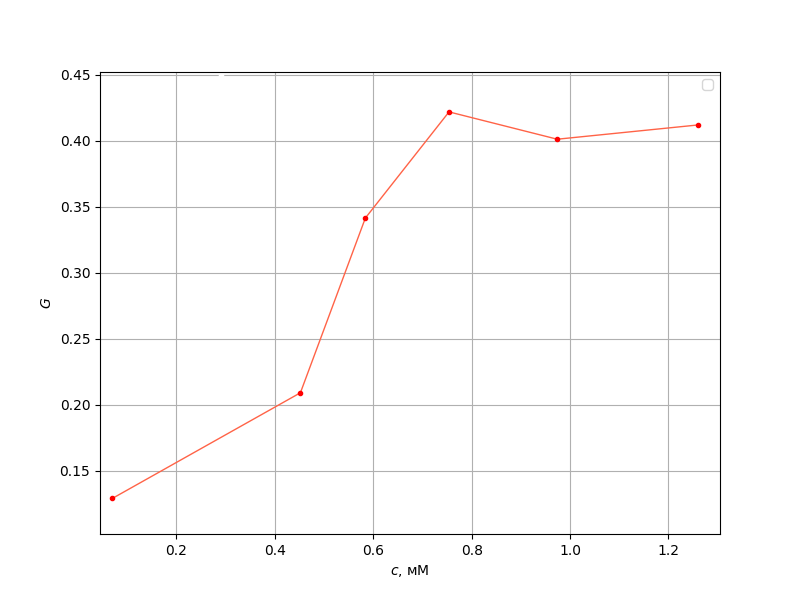
\includegraphics[width = 0.8\textwidth]{G_cc.png}
    \caption{Зависимость поверхностного избытка Гиббса от концентрации. }
\end{figure}\\
\newpage
В предположении адсорбции Ленгмюра (\ref{ленгмюр})
\begin{equation*}
    \text{Г} = \text{Г}_{\infty}\frac{KC}{KC + 1}
\end{equation*}
Тогда 
\begin{equation*}
    \frac{1}{\text{Г}} = \frac{1}{\text{Г}_{\infty}} (1 + \frac{1}{KC})
 \end{equation*}
\begin{equation} \label{aaa}
    \frac{C}{\text{Г}} = \frac{C}{\text{Г}_{\infty}} + \frac{1}{K\text{Г}_{\infty}}
\end{equation}
Построим изотерму адсорбции в линеаризующих координатах $\frac{1}{\text{Г}} = f(\frac{1}{C})$ и найдем из графика $\text{Г}_{\infty}$ и $K$

\begin{table}[h!]
\centering
\begin{tabular}{|c|r|r|}
\hline
№ & \multicolumn{1}{l|}{$c$, мМ} & \multicolumn{1}{l|}{$\frac{c}{G}, \frac{10^{6} }{м}$} \\ \hline
1 & 0.584                        & 0.2414                                                \\ \hline
2 & 0.452                        & 0.2090                                                \\ \hline
3 & 0.07                         & 0.1290                                                \\ \hline
\end{tabular}
\caption{Избыток Гиббса в зависимости от концентрации ПАВ в линеаризующих координатах.}
\label{tab:my-table}
\end{table}


\newpage
\begin{figure}[h!]
    \centering
    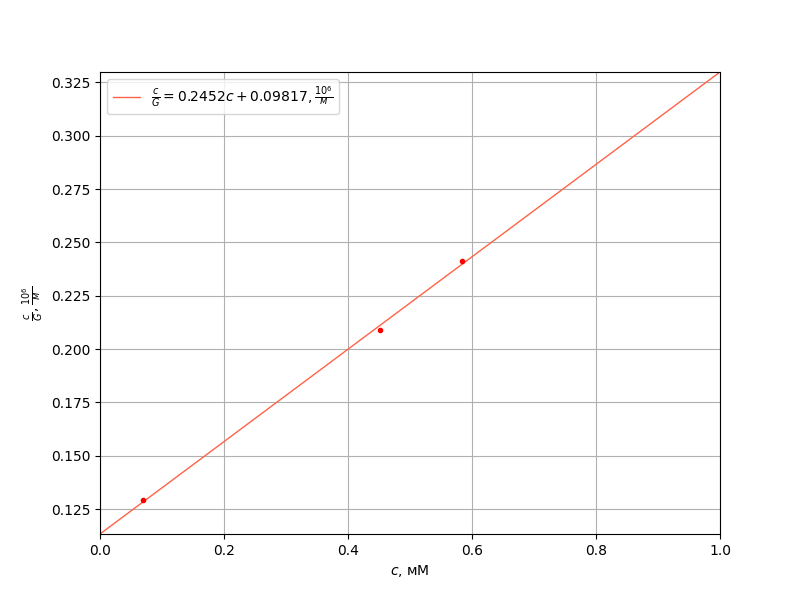
\includegraphics[width = 0.8\textwidth]{c_G_line_end.png}
    \caption{Зависимость адсорбции от концентрации в линеаризующих координатах}
\end{figure}\\

С учетом формулы (\ref{aaa}) и МНК
\begin{equation*}
    \text{Г}_{\infty} = \frac{1}{0.2452}\frac{10^{-6}\text{моль}}{\text{м}^2} = 4.07\cdot 10^{-6}\frac{\text{моль}}{\text{м}^2}
\end{equation*}

\begin{equation*}
    \frac{1}{K} = \frac{0.2452}{0.0982}\cdot 10^{3} \text{М}
\end{equation*}
\begin{equation*}
    K \approx 2498 \text{М}^{-1}
\end{equation*}
Предельная адсорбция сравнима с получившейся при апроксимации пределльного участка, однако они не совпадают. Различия могли возникнуть из-за того, что в данном расчете брались дискретные производные, не равные обычным (т.е. было недостаточно данных для более точного расчета), а также аппроксимация проводилась лишь по двум точкам в силу быстрого заполнения монослоя адсорбирующемся веществом (линейный участок на кривой зависимости поверхностного натяжения от концентрации в полулогарифмических координатах). В первом методе определения предельной адсорбции точек было достаточно, так как там уже сформировался насыщенный монослой и кривая адсорбции стала прямой. Исходя из этих рассуждений можно сделать вывод о том, что значение $ \text{Г}_{\infty}$, полученное в первом случае, более достоверно, чем во втором.
 
\item
Расчитаем стандартную свободную энергию адсорбции
\begin{equation*}
    \Delta G^{\circ} = - RTlnK = - 8.31\cdot298\cdot ln(2498) = -19.4  \text{кДж/моль}
\end{equation*}
Для оценки полученного результата воспользуемся правилом Дюкло-Траубе для ионогенных ПАВ
\begin{equation*}
    \frac{g_{n+1}}{g_{n}} = 2.1
\end{equation*}
где $g_{n} = -\frac{d\sigma}{dC}$ при $C\rightarrow0$ для n-го гомолога ПАВ\ 
Из уравнения Гиббса при $C\rightarrow0$
\begin{equation*}
    \text{Г} = -\frac{C}{RT}\frac{d\sigma}{dC} = \frac{C}{RT} g
\end{equation*}
Значит, 
\begin{equation*}
    \frac{\text{Г}_{n+1}}{\text{Г}_{n}} = \frac{g_{n+1}}{g_{n}} = 2.1
\end{equation*}
При $C\rightarrow0$ уравнение адсорбции Ленгмюра переходит в уравнение адсорбции Генри 
\begin{equation*}
    \text{Г} = KC
\end{equation*}
Тогда 
\begin{equation*}
    \frac{K_{n+1}}{K_{n}} = 2.1
\end{equation*}
Найдем разность стандартных энергий адсорбции для соседних гомологов ПАВ
\begin{equation*}
    \delta = \Delta G_{n+1}^{\circ} - \Delta G_{n}^{\circ} = - RT\ln{K_{n+1} }+ RT\ln{K_{n}} = RT\ln{\frac{K_{n}}{K_{n+1}}} \approx -1.84 \frac{\text{кДж}}{\text{моль}}
\end{equation*}
Считаем, что $\Delta G_{0}^{\circ} = 0$, тогда $\Delta G_{n}^{\circ} = n\delta$.
Тогда для TTAB c $n = 14$
\begin{equation*}
    \Delta G_{14}^{\circ} = n\delta = 14\cdot(-1.84) = -25.72\frac{\text{кДж}}{\text{моль}}  \approx -26\frac{\text{кДж}}{\text{моль}}
\end{equation*}\

Таким образом, экспериментальный результат и теоретическая оценка согласуются друг с другом(погрешность расхождения результата - 27 \%). Разница могла возникнуть из-за того, что оценка производится при $c\rightarrow0$, в то время как экспериментальный расчет - при конечных небольших концентрациях.


\end{enumerate}

\section{Обсуждение результатов и выводы}
\begin{itemize}

\item Определение ККМ в растворе ПАВ кондуктометрическим методом показало довольно точные результаты, практически совпадающие с табличными. При измерениях наибольший вклад в погрешность могло внести приготовление растворов.

\item Определение ККМ в растворе ПАВ методом определения поверхностного натяжения существенно менее точен, так как очень сложно избавиться от примесей в растворе ПАВ, которые из-за лучшей адсорбции уменьшают поверхностное натяжение, что приводит к минимуму на изотерме поверхностного натяжения. В результате мы не имеем чёткого излома, по которому можно точно определить ККМ и можем лишь очень приблизительно оценивать это значение.

\item В процессе работы были произведены: оценка длины молекулы ПАВ в монослое $l_{scaled} = 2.186$ нм, $l_{exp} = 1.38$ нм, оценка стандартной свободной энергии адсорбции $ \Delta G^{\circ}_{scaled} = -26$ кДж/моль, $ \Delta G^{\circ}_{exp} = -19.4 $ кДж/моль. Были полученны значения для константы адсорбции: $K \approx 2498 \text{М}^{-1}$, предельного избытка Гиббса:  $\text{Г}_{\infty}_{1} =  5.39 \cdot 10^{-6} \frac{\text{моль}}{\text{м}^{2}}, \text{Г}_{\infty}_{2} = 4.07 5.39 \cdot 10^{-6} \frac{\text{моль}}{\text{м}^{2}}$, площадь, приходящуюся на одну молекулу: $ S_{0} = 3.08\cdot10^{-19}\text{м}^{2}$.

\end{itemize}














\newpage

\addcontentsline{toc}{section}{Список используемой литературы}
\begin{thebibliography}{}
    \bibitem{1}  Департамент химии МФТИ -  "Адсорбция и мицеллообразование в растворах ПАВ: определение ККМ по измерению электропроводности и поверхностного натяжения"
    \bibitem{2}  Лекции по теории элементарного акта химических реакций в конденсированной фазе, Москва 2000 - https://www.chem.msu.su/rus/teaching/vorob'ev/pril.html
\end{thebibliography}



\end{document}
